\section{Part 4: Heuristics in the Adaptive A* }
\label{sec: Part 4}

In our grid world, we are operating with an atomic unit where each cell is the atom. In our grid world, we can only move in the main compass directions of north, south, west, and east. This means that the shortest distance between two cells is always the $Manhattan Distance$. This simply means that if we have 2 points, $p_1(x_1,y_1)$ and $p_2(x_2,y_2)$, then the Manhattan Distance between them is given by  $D = |x_2 - x_1| + |y_2 - y_1|$. 


In order for \emph{$A^*$ search} to work properly, it requires a consistent heuristic. A consistent heuristic is defined as one that has the distance from the current node to the goal as always less than or equal to distance from any neighbor node to the goal plus the distance to reach that neighbor. In other words, assume $n$ is any node on the grid, then $h(n) \leq c(n,p) + h(p)$, where $h(n)$ is our heuristic value of node $n$, $c(n,p)$ is the distance from node $n$ to one other node $p$, and $h(p)$ is the heuristic value of node $p$. Of course, using simple geometry, this must always be true when dealing with euclidean distances, as shown below.
\begin{figure}[H]
  \centering
  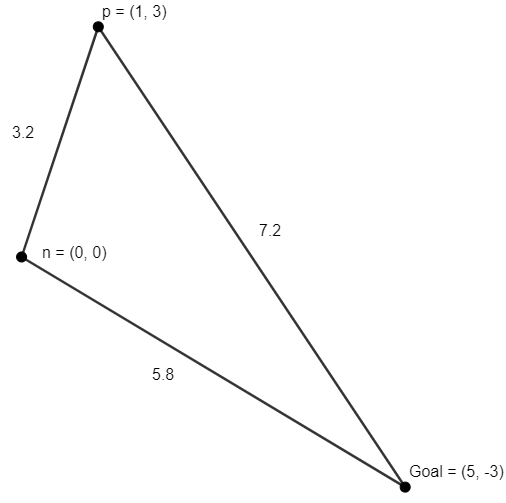
\includegraphics[width=0.5\linewidth]{Report/Part4/Annotation 2020-07-10 224338.png}  
\caption{Consistent heuristics with Euclidean Distance}
\end{figure}

We can observe that the heuristic above is admissible since $h(n) \leq c(n,p) + h(p)$ holds. In other words, $5.8 \leq 3.2 + 7.2$ due to the triangle inequality. Namely, it is impossible to have a triangle where the length of the sum of 2 sides is larger than the third side. Now we will prove this for the case of Manhattan Distances.


\linebreak
\begin{qoute}
\emph{Prove that Manhattan distances are consistent in
grid worlds in which the agent can move only in the four main compass directions.}
\end{qoute}
\begin{proof}
Assume for contradiction that Manhattan distances are not consistent. This means that $\forall n, h(n) > c(n,p) + h(p)$. Lets assume we have cells, $q_1(x_1,y_1)$, $q_2(x_2,y_2)$ and $q_3(x_3,y_3)$, where $q_2 \in q_1_{neighbors}$ and $q_3$ is our goal. Then, by letting $n = q_1$ and $p = q_2$, we deduce that the distance between these 2 cells is given by $D = |x_2 - x_1| + |y_2 - y_1|$. By substitution, our new inequality for $h(n)$ becomes $\{|x_3 - x_1| + |y_3 - y_1|\} > \{|x_2 - x_1| + |y_2 - y_1|\} + \{|x_2 - x_3| + |y_2 - y_3|\}$. To make sense of this, we can realize that any 3 points form a triangle in the euclidean world, and a rectangle in the Manhattan world, as shown below.
\begin{figure}[H]
  \centering
  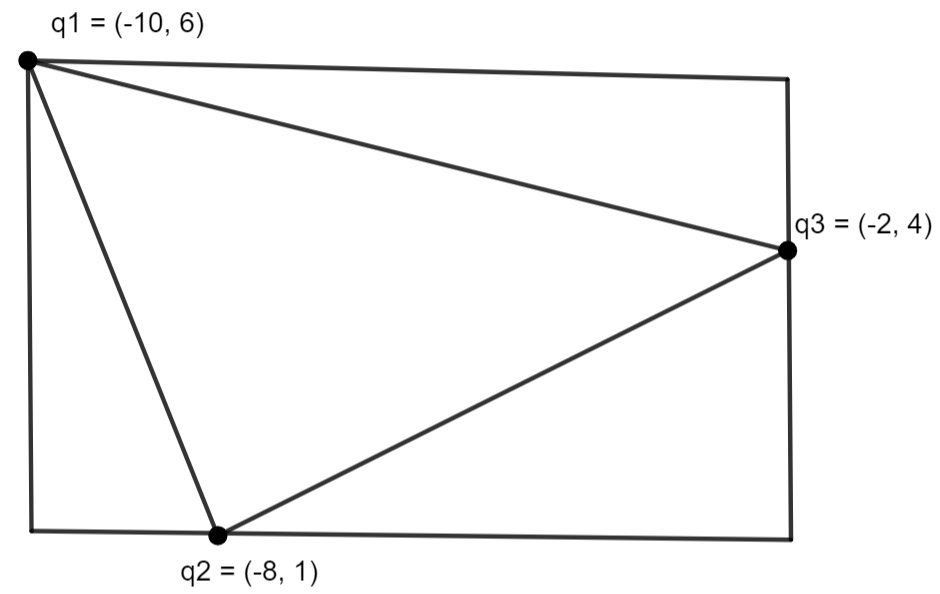
\includegraphics[width=0.5\linewidth]{Report/Part4/Capture.PNG}  
\caption{3 Points in Manhattan World}
\end{figure}

This means that by the triangle inequality, the distance between any two points is must be greater than the straight line distance. In fact, now we can take $\{|x_3 - x_1| + |y_3 - y_1|\} > \{|x_2 - x_1| + |y_2 - y_1|\} + \{|x_2 - x_3| + |y_2 - y_3|\}$ and compute where each section in brackets corresponds to on the rectangle. $|x_3 - x_1| + |y_3 - y_1|$ corresponds to the 2 legs formed from $q_1 \rightarrow q_3$. Then, $|x_2 - x_1| + |y_2 - y_1|$ corresponds to the legs formed from $q_1 \rightarrow q_2$ and $|x_2 - x_3| + |y_2 - y_3|$ is the legs of $q_2 \rightarrow q_3$. Now, we can further analyze the fact that the longest 2 legs possible, will form only half of the rectangle, meaning, our 3 points form a right triangle. With this in mind, we can look at our original inequality, $\{|x_3 - x_1| + |y_3 - y_1|\} > \{|x_2 - x_1| + |y_2 - y_1|\} + \{|x_2 - x_3| + |y_2 - y_3|\}$ and realize it muse be a contradiction! It is not possible for the length of 2 legs of a triangle to form more than half of the rectangle, and therefore, $\{|x_3 - x_1| + |y_3 - y_1|\} \leq \{|x_2 - x_1| + |y_2 - y_1|\} + \{|x_2 - x_3| + |y_2 - y_3|\}$. Therefore, Manhattan distances are consistent in grid worlds where the agent can move only in the four main compass directions.
\end{proof}


Our next concern will be with a variant of \emph{$A^*$ search} known as \emph{Adaptive $A^*$ search}. The idea behind this variant will be explained in more detail in the next section, but the main difference is that for an \emph{online search} problem, \emph{Adaptive $A^*$ search} will update the heuristic values of all the expanded nodes after each $A^*$ call. Remember, $A^*$ will only work with consistent heuristic values, therefore, this raises the question if our heuristic values are still consistent after updating them.

\begin{qoute}
\emph{Prove that Adaptive $A^*$ leaves initially consistent h-values consistent even if action costs can increase.}
\end{qoute}
\begin{proof}
After each \emph{$A^*$ search} we update our heuristics given by the function $h_{new}(s) = g(goal) - g(s)$. By doing so, we will always have an admissible heuristic since our $A^*$ path length is always optimal. Now, using the definition of a consistent heuristic, $h(s) \leq c(s,p) + h(p)$, we can substitute in $h_{new}(s)$ and $h_{new}(p)$ and obtain $g(goal) - g(s) \leq c(s,p) + g(goal) - g(p)$. By further simplification, $g(p) \leq c(s,p) + g(s)$. We then realize that this inequality looks very familiar, in fact, it is just our original $h(s) \leq c(s,p) + h(p)$ with the goal and start nodes reversed. We proved in the previous part that Manhattan distances were consistent in grid worlds with moving only in the 4 main compass directions, and the same proof applies for this inequality as well, with the difference being the start and goal nodes are switched.
\end{proof}

